\documentclass{article}
\usepackage{float}
\usepackage{graphicx}
\usepackage{caption}
\usepackage{placeins}
\usepackage{textcomp}

\title{Quality Threshold Clusteing}
\date{20-03-2020}
\author{Ivan Diliso Matricola: 676366}

\graphicspath{ {./Images/} }
\captionsetup{justification=raggedright,singlelinecheck=false}


\begin{document}
    
    \maketitle
    \tableofcontents
    \newpage
    \section{Introduzione}
    Il software \textbf{Qt-Clustering} realizzato in Java permette di applicare 
    l'algoritmo di cluster Quality Threshold ad un insieme di dati estratti da 
    un database MySQL. 

    \paragraph{Quality Threshold} 
    Algoritmo alternatico per partizionare i dati. Richiede piu' potenza di
    calcolo rispetto a K-Means ma non richiede di specificare il numero di
    cluster a priori, e restituisce sempre lo stessorisultato quando si ripete
    diverse volte.
 
    \section{Applicazione principale}
    L'applicazine e' divisa in due componenti principali
        \subsection{Server}
        Il server si occupa di eseguire le richieste di uno o piu client
        fornendo ad essi le seguenti funzionalita:
            \begin{itemize}
                \item Caricare una tabella dal database specificandone il nome
                \item Eseguire il clustering dei dati caricati con un raggio
                specificato dall'utente
                \item Visualizzare i dati e il risultato del clustering
                \item Salvare il risultato del clustering su file
                \item Caricare i dati del clustering da file
            \end{itemize}
        
        
        \subsection{Client}
        Il client si occupa di gestire una interaccia utente basata su linea di 
        comando che permette all'utente di:
            \begin{itemize}
                \item Connettersi al server specificando una porta (valore di 
                default 8080)
                \item Chiedere al server di eseguire una nuova operazione di
                clustering specificando nome della tabella, raggio e io nome del
                file dove salvare i risultati
                \item Caricare un clustering salvato su file specificando il
                nome del file
            \end{itemize}

    \newpage
    \section{Estensione}
    L'estenzione del progetto consiste su una Web Application basata sul
    framework Spring Boot, che permette di creare applicazioni web basate sul
    pattern architetturale MVC (Model View Controller). 
    L'applicazione e' basata sull'utilizzo di servlet per servire le pagine web,
    non sara' piu' presente dunque un modello client server basato su socket ma 
    il client sara' rappresentato da una pagina web che si interfaccera con il
    server per l'esecuzione del clustering, il caricamento dei dati dal database 
    e il trasferimento dei dati.

        \paragraph{Servlet}
        Oggeto scritto in linguaggio Java che opera all'interno di
        un server web permettendo quindi la creazine di applicazioni web.
    
        \subsection{Web Server}
        E' stata utilizzata una versione che opera tramite il web server e 
        servlet container Tomcat embedded all'interno dell'applicazione. 
        In questo modo non ci sara' bisogno di avviare il web server Tomcat ma 
        bastera' avviare il WAR (Web Application Resource) del server per 
        avviare sia il web server, sia la web application

        \subsection{Libreria JSON}
        Per servire i dati del database e i risultati del clustering sono state
        create delle classi per la costruzione di file JSON. La libreria
        presenta una struttura ad albero per rappresentare i dati.

        \subsection{Frontend}
        Il frontend e' stato realizzato in HTML/CSS e presenta delle funzoni 
        in Javascript per trasformare i dati JSON forniti dal server in tabelle
        HTML. E' stata utilizzata la libreria BOOTSTRAP per omoloagare la 
        grafica delle pagine web e fornire dei siti web responsive. \\\\
        Sono state aggiunte delle funzioni (sia backend, sia frontend)
        per permettere di visualizzare l'elenco delle tabelle 
        presenti nel database e selezionare la tabella 
        tramite un menu a tendina






    \newpage
    \section{Installazione}
    Questi passaggi sono validi sia per il progetto base sia per il progetto con
    estensione.
    Sia il client sia il server necessitano l'installazione dei sequenti
    software:
        \begin{itemize}
            \item MySQL
            \item Java Runtime Envrioment 8.0
        \end{itemize}

        \subsection{Server}
            \begin{enumerate}
                \item Accertarsi che il server MySQL sia attivo sulla propria
                macchina
                \item Eseguire il file SQL databasesetup.sql tramite il comando:
                    \\\\
                    \verb|mysql -u root -p < databasesetup.sql|
                
                
            \end{enumerate}

        \subsection{Client}
        Il client sia nel progetto base sia nel progetto con estensione non
        richiedono particolari passaggi per l'installazione
    
    \section{Manuale Utente}
        
            \subsection{Client}
            Avviare il client facendo doppio click sul file 
            \verb|Client.bat| in questo caso verranno utilizzati indirizzo
            IP e porta di default (localhost:8080). Per specificare un
            diverso indirizzo ip e port usare il comando: \\\\
            \verb|QtClient.bat <ip> <porta>|

            \subsection{Server}
            Avviare il server facendo doppio click sul file 
            \verb|Server.bat| in questo caso verra' utilizzata la porta di
            default (8080). Per specificare una diversa porta 
            usare il comando: \\\\
            \verb|QtServer.bat <porta>|\\\\
            I file creati dal server verranno salvati nella stessa cartella
            in cui e' contenuto il file bat
            
            \subsection{Server Estensione}
            Avviare il server facendo doppio click sul file 
            \verb|WebServer.bat| in questo caso verra' utilizzata la porta di
            default (8080). Per specificare una diversa porta 
            usare il comando: \\\\
            \verb|QtWebServer.bat <porta>|\\\\
            I file creati dal server verranno salvati nella stessa cartella
            in cui e' contenuto il file bat
            
            \subsection{Client Estensione}
            Accedere al sito web alla pagina: \\\\
            \verb|https://localhost:8080/index|


    \section{Esempi utilizzo}
            \subsection{Progetto Base}
    In tutte le immagini le parole in verde sono input forniti dall'utente

        \begin{figure}[!ht]
            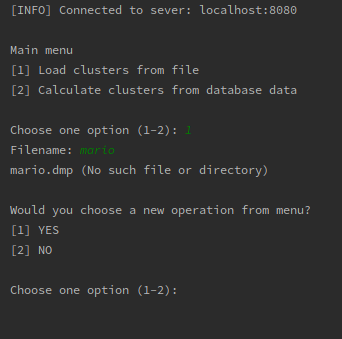
\includegraphics{BASE1}
            \caption{L'utente sceglie di caricare i risultati del clustering 
            da file. Prova quindi a caricare un file chiamato "mario" ma il file non
            e' presente quindi viene visualizzato un errore. All'utente viene
            chiesto se vuole scegliere una nuova opzione dal menu}   
            \label{fig:1}
        \end{figure}

        \begin{figure}[!ht]
            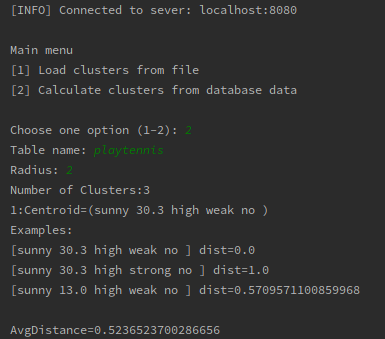
\includegraphics{BASE2}
            \caption{L'utente sceglie di effettuare il clustering su tabella su
            database, inserisce quindi il nome della tabella e il raggio. Nell'
            immagine viene visualizzato solo uno dei tre cluster forniti in output.}   
            \label{fig:2}
        \end{figure}

        \begin{figure}[H]
            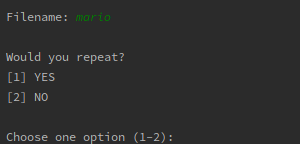
\includegraphics{BASE4}
            \caption{Dopo aver visualizzato i risultati viene chiesto all'
            utente di inserire il nome del file in cui salvare i risultati. L'
            utente puo' decidere di effetuare nuovamente la computazine sulla
            stessa tabelle fornendo soltanto il raggio.}   
            \label{fig:3}
        \end{figure}


        \begin{figure}[H]
            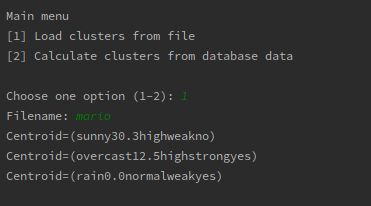
\includegraphics{BASE5}
            \caption{Scegliendo di caricare i cluster da file e inserendo un 
            nome di file corretto vengono visualizzati i dati dei cluster.}   
            \label{fig:4}
        \end{figure} 
        \FloatBarrier
       
 



    \subsection{Estensione}
    E' stato utilizzato il browser Firefox per le prove di utilizzo della 
    applicazione web


    \begin{figure}[H]
        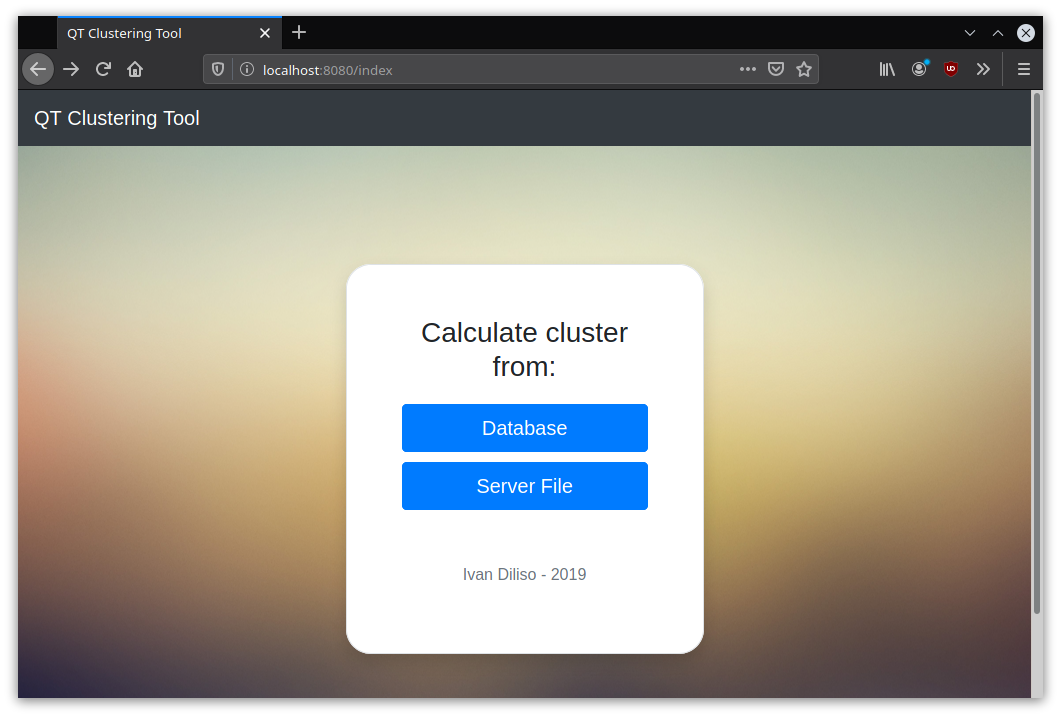
\includegraphics[scale=0.4]{ADDON1}
        \caption{Menu principale, per caricare effettuare il clustering su 
        database cliccare il pulsante "Database", per caricare i risultati del
        clustering da file cliccare il pulsante "Server File"}   
        \label{fig:5}
    \end{figure} 
    \begin{figure}[H]
        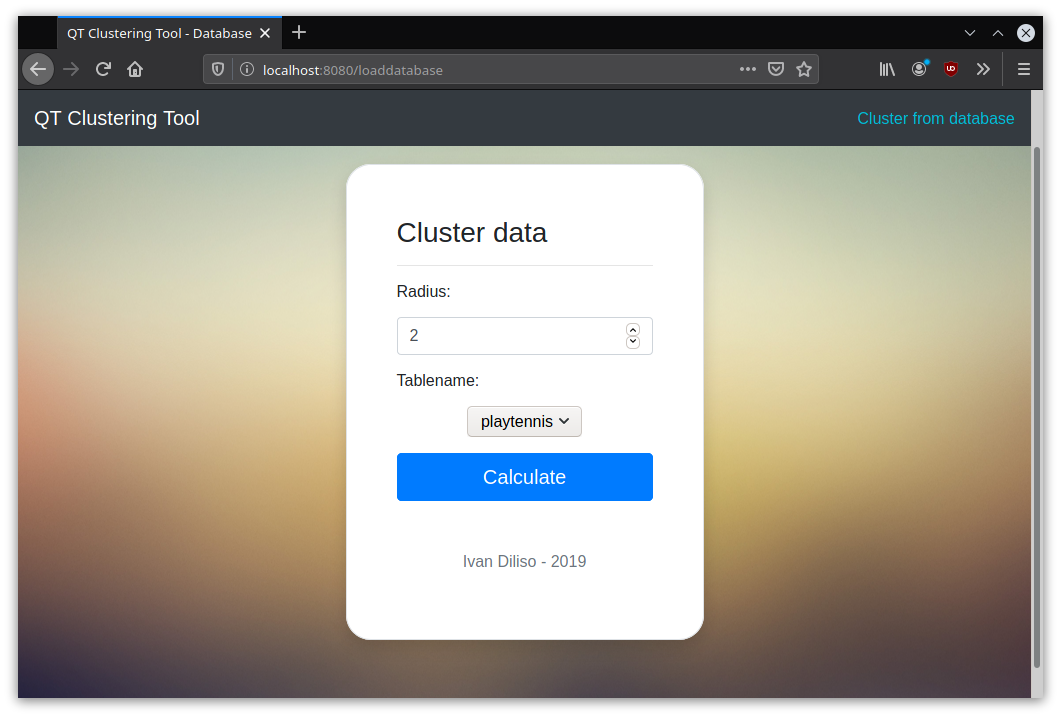
\includegraphics[scale=0.4]{ADDON2}
        \caption{Cliccando il pulsante "Database" si arriva su questa pagina. L'
        utente ha inserito un raggio e ha selezionato dal menu a tendina 
        la tabella da caricare. }   
        \label{fig:6}
    \end{figure} 
    \begin{figure}[H]
        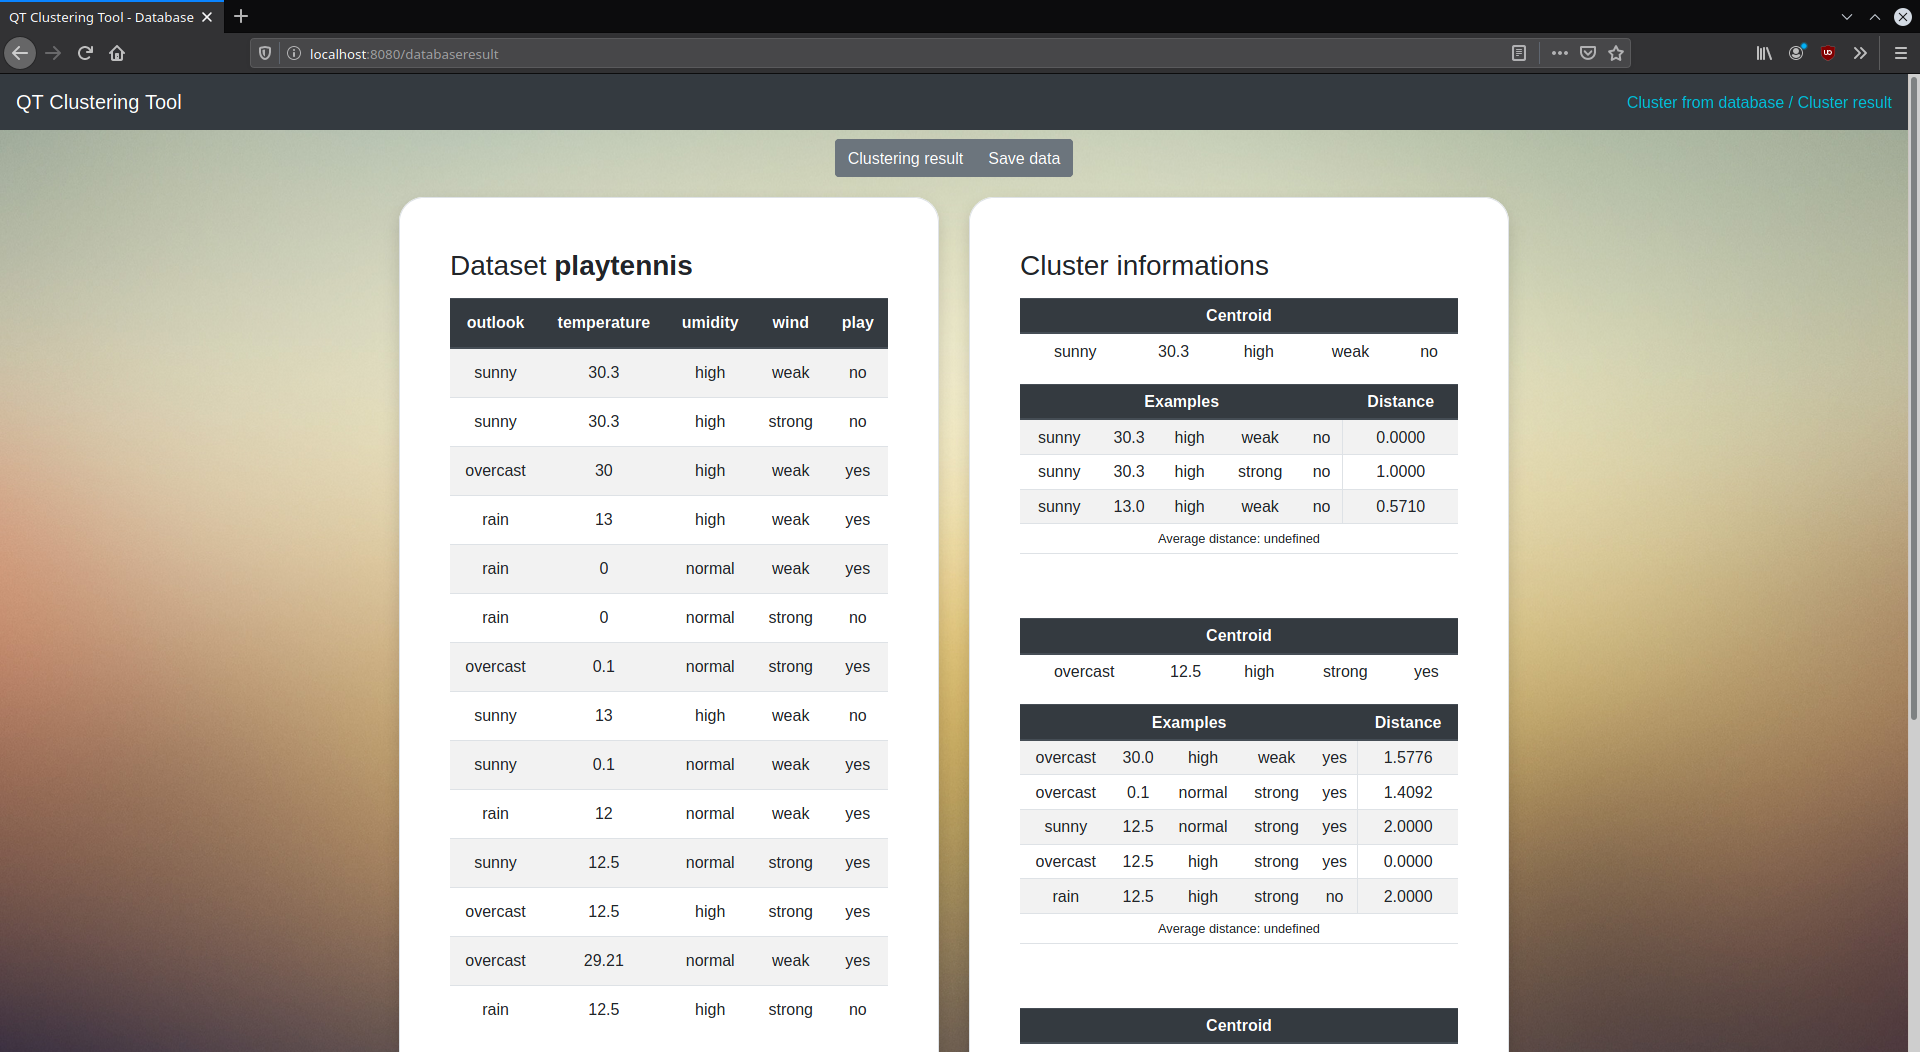
\includegraphics[scale=0.3]{ADDON3}
        \caption{Vengono visualizzati i risultati del clustering. Cliccare su 
        "Save Data" per salvare i risultati su file}   
        \label{fig:7}
    \end{figure} 
    \begin{figure}[H]
        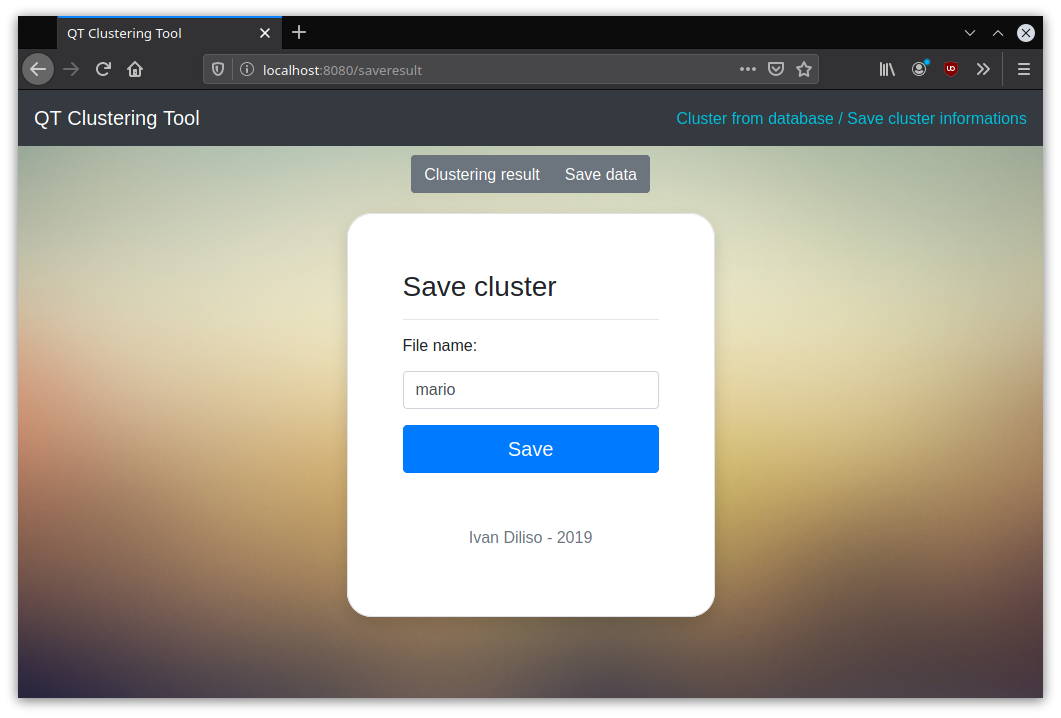
\includegraphics[scale=0.4]{ADDON4}
        \caption{L'utente inserisce il nome del file sul quale salvare i 
        risultati del clustering}   
        \label{fig:8}
    \end{figure} 
    \begin{figure}[H]
        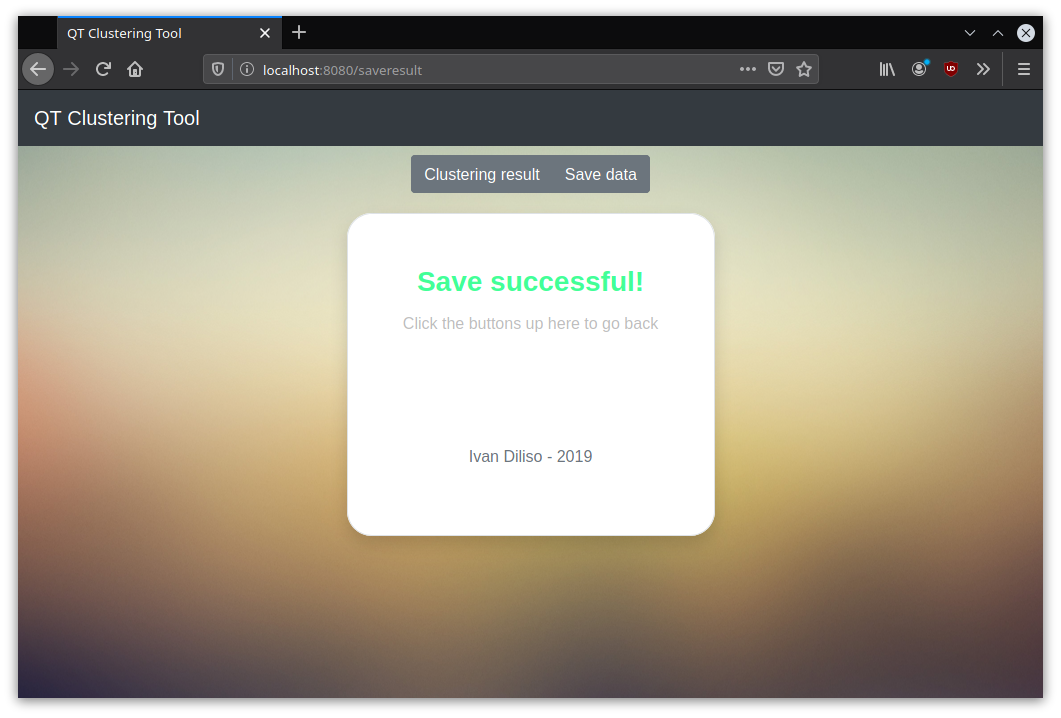
\includegraphics[scale=0.4]{ADDON5}
        \caption{Salvataggio su file avvenuto con successo}   
        \label{fig:9}
    \end{figure} 
    \begin{figure}[H]
        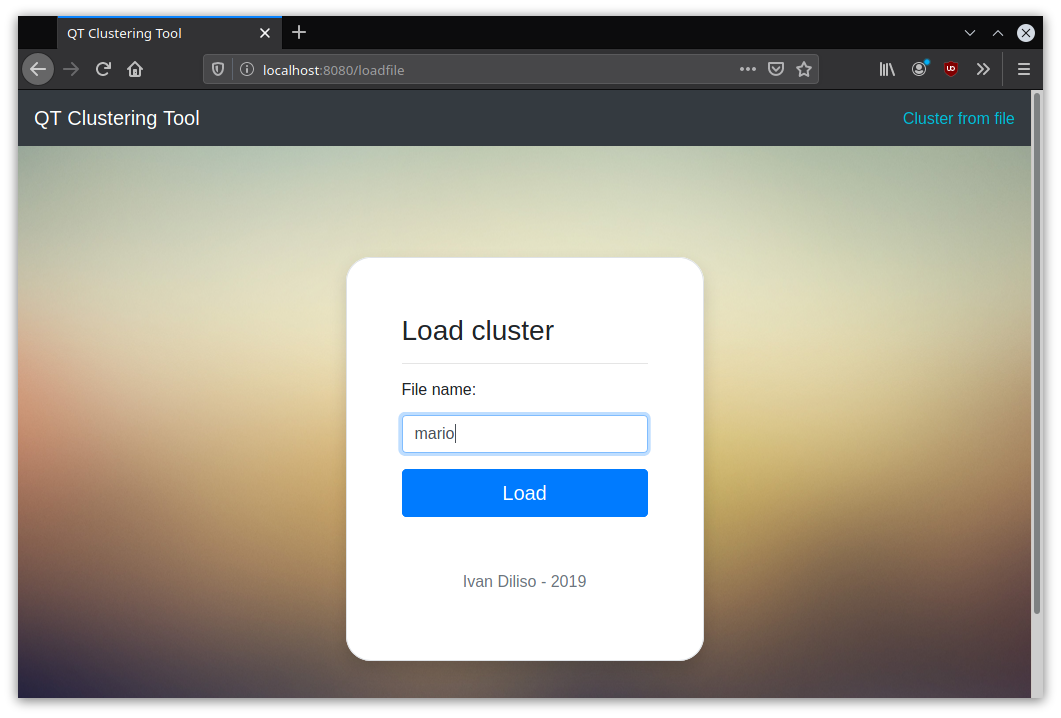
\includegraphics[scale=0.4]{ADDON6}
        \caption{Cliccando su "Server File" nel menu principale si arriva 
        a questa pagina. L'utente inserisce il nome del file dal quale 
        caricare i dati del clustering}   
        \label{fig:10}
    \end{figure} 
    \begin{figure}[H]
        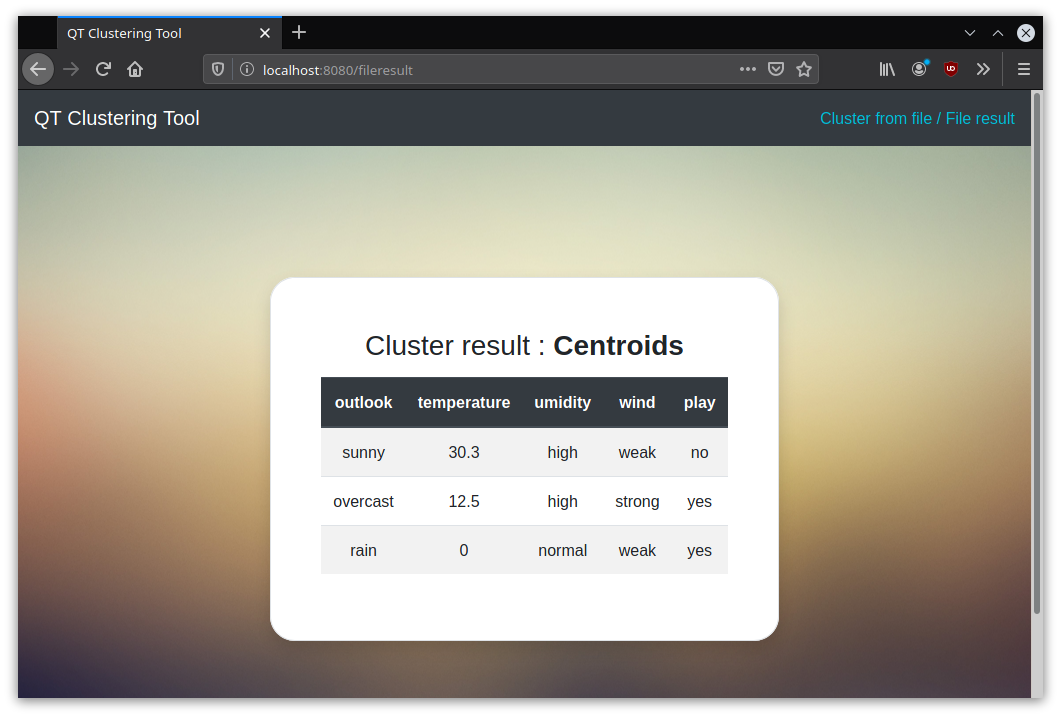
\includegraphics[scale=0.4]{ADDON7}
        \caption{Dati del clustering caricati da file.}   
        \label{fig:11}
    \end{figure} 
    \begin{figure}[H]
        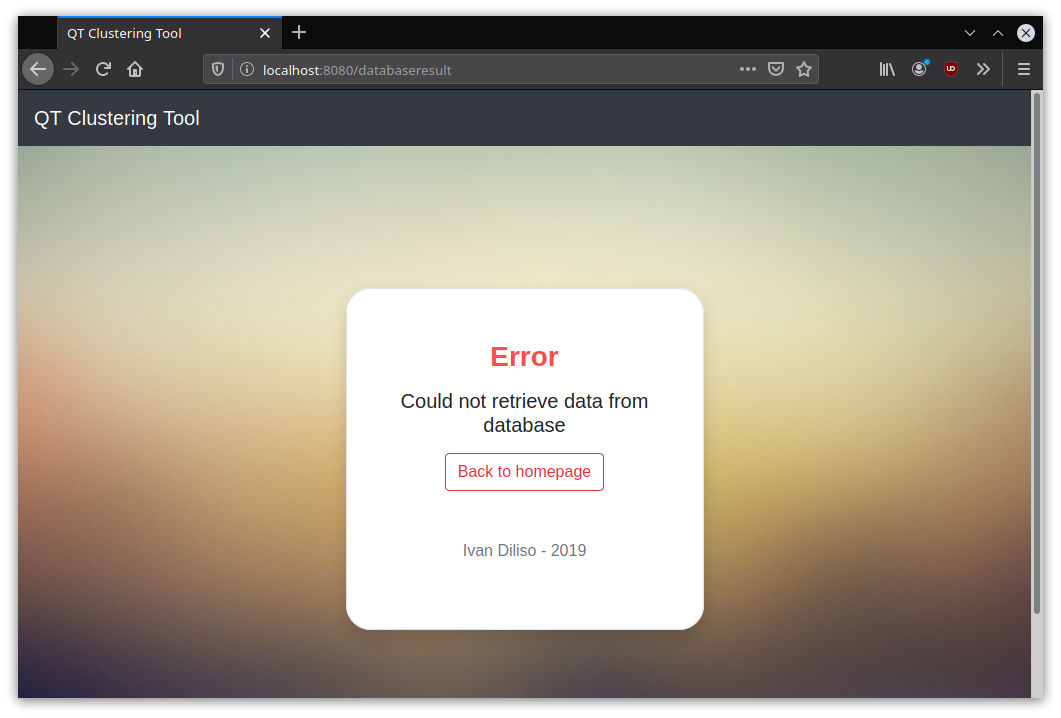
\includegraphics[scale=0.4]{ADDON8}
        \caption{Pagina in cui vengono visualizzati eventuali errori del 
        server. Cliccare sul pulsane "Back to Homepage" per tornare alla 
        Homepage}   
        \label{fig:12}
    \end{figure} 


    \section{Note}
    Nello sviluppo del progetto e' stato utilizzato il software 
    \textbf{Git} per il controllo di versione e il software 
    \textbf{Gradle} come sistema di build e gestore delle dipendenze \\\\
    Sono presenti due tabelle per il test dell'applicazione \verb|playtennis| 
    e \verb|testtable|
        \subsection{Importare il progetto in Eclipse}
        File $>$ Import $>$ Gradle $>$ Existing Gradle Projet $>$ Next $>$
        Selezionare la cartella QtClient / QtServer / QtWebServer $>$ Next $>$
        Finish
        \subsection{Importare il progetto in IntelliJ  Idea}
        Import Projct $>$
         Selezionare la cartella QtClient / QtServer / QtWebServer 
         $>$
        Import project from external model $>$ Selezionare Gradle $>$ Finish 

        \subsection{Compilare l'applicazione}
        Utilizzare il task Gradle "build" per compilare l'applicazione, 
        utilizzare il task "run" per avviare l'applicazione.

\end{document}